%%%%%%%%%%%%%%%%%%%%%%%%%%%%%%%%%%%%%%%%%%%%%%%%%%%%%%%%%%%%%%%%%%%%%%
% How to use writeLaTeX: 
%  
% You edit the source code here on the left, and the preview on the
% right shows you the result within a few seconds.
%
% Bookmark this page and share the URL with your co-authors. They can
% edit at the same time!
%
% You can upload figures, bibliographies, custom classes and
% styles using the files menu.
%
%%%%%%%%%%%%%%%%%%%%%%%%%%%%%%%%%%%%%%%%%%%%%%%%%%%%%%%%%%%%%%%%%%%%%%

\documentclass[12pt]{article}

\usepackage{sbc-template}

\usepackage{graphicx,url}

\usepackage[brazil]{babel}   
\usepackage[utf8]{inputenc}

     
\sloppy

	
%Daniella Martins Vasconcellos (Universidade do Estado de Santa Catarina)
%Guilherme Tomaselli Borchardt (Universidade do Estado de Santa Catarina)
%Laís Pisetta Van Vossen (Universidade do Estado de Santa Catarina)
%Maria Teresa Silva Santos (Universidade do Estado de Santa Catarina)
%Eric Carvalho da Silveira (Universidade do Estado de Santa Catarina (UDESC))
%Carlos Daniel Schmitt Bunn (Universidade do Estado de Santa Catarina)
%Isabela Gasparini (Universidade do Estado de Santa Catarina (UDESC))

\renewcommand{\email}[1]{\\\mbox{}\\[-6pt]\footnotesize\ttfamily\begin{tabular}{@{} c @{}}#1\end{tabular}}

\title{Estudos sobre evasão em diferentes ambientes educacionais e seus relacionamentos com gênero e a diversidade}

% \title{Estudos sobre a evasão no Brasil e seus relacionamentos com gênero e a diversidade}
%=====COLOCAR AGRADECIMENTOS========
\author{
Daniella Martins Vasconcellos$^1$,
Guilherme Tomaselli Borchardt$^1$,\\
Laís Pisetta Van Vossen$^1$,
Maria Teresa Silva Santos$^1$, \\ 
Eric Carvalho da Silveira$^1$,
Carlos Daniel Schmitt Bunn$^1$,\\
Isabela Gasparini$^1$}

%=====COLOCAR AGRADECIMENTOS========
\address{Universidade do Estado de Santa Catarina, Joinville, Santa Catarina, Brasil
  %=====COLOCAR AGRADECIMENTOS========
  \email{\{daniella.vasconcellos, guilherme.borchardt, lais.vossen, \\ maria.santos2805, eric.silveira,  carlos.bunn\}\\ @edu.udesc.br, isabela.gasparini@udesc.br}
}

\begin{document}
\maketitle

\begin{abstract}
The analysis of educational data is essential for understanding the academic context and supporting the creation of public policies. This work presents: (1) a systematic mapping on dropout prediction; (2) a questionnaire to identify possible reasons for dropout; (3) a proposal for an educational data visualization tool; (4) an analysis of female dropout rates in computer science courses in Santa Catarina; (5) an overview of diversity in computer science courses at public universities in Santa Catarina; (6) a collaborative tool for dropout prediction in disciplines. These studies are relevant in the field of computer science as they address academic issues and contribute to the development of prediction systems and policies to reduce dropout rates.

% The analysis of educational data is essential to understand the academic context and support the creation of public policies in Brazil. This work presents: (1) a systematic mapping on dropout prediction; (2) a questionnaire to identify possible reasons for dropout; (3) a proposal for an educational data visualization tool; (4) an analysis of female dropout in computer science courses in Santa Catarina; (5) an overview of diversity in computer science courses at public universities in Santa Catarina. These studies are relevant in the field of computer science as they report issues in the academic community and can be used as a basis for proposed prediction systems and institutional policies to reduce dropout rates.
\end{abstract}
     
\begin{resumo} 
A análise de dados educacionais é essencial para entender o contexto acadêmico e apoiar a criação de políticas públicas. Este trabalho apresenta: (1) mapeamento sistemático sobre predição da evasão; (2) questionário para identificar possíveis motivos de evasão; (3) proposta de ferramenta de visualização de dados educacionais; (4) análise da evasão feminina nos cursos de computação em Santa Catarina; (5) panorama da diversidade nos cursos de computação das universidades públicas de Santa Catarina; (6) ferramenta colaborativa para predição de evasão nas disciplinas. Esses estudos são relevantes na área de computação, pois abordam problemas acadêmicos e contribuem para propostas de sistemas de predição e políticas de combate à evasão.
\end{resumo}


\section{Introdução}
\label{sec:introducao}

Análises de dados educacionais são importantes para a sociedade por possibilitar um melhor entendimento sobre o contexto educacional e também para a criação de medidas que visam melhorar todos os níveis da educação. No Brasil, a entidade responsável por esses dados é o Instituto Nacional de Estudos e Pesquisas Educacionais Anísio Teixeira (INEP), a qual, de forma anual, disponibiliza em seu próprio portal as bases de dados educacionais, que podem ser utilizadas em pesquisas abordando diversos aspectos e também para auxiliar o desenvolvimento de políticas públicas. 

Contudo, segundo Macedo et al. (2020)\nocite{macedo2020ferramenta}, em função das grandes quantidades de dados educacionais que são gerados anualmente, a exploração e a realização de análises sobre esses dados ainda é um desafio para boa parte da população. Já para Davenport e Patil (2012)\nocite{davenport2012data}, a habilidade de conseguir trabalhar com dados educacionais é essencial, pois as instituições de ensino estão gerando enormes volumes de dados, e a capacidade de analisar esses dados pode contribuir para nortear a sociedade nas tomadas de decisões mais assertivas. 

Com isso, introduz-se o grupo de iniciação científica focado em estudos relacionados à evasão, composto por cinco estudantes da graduação em Bacharelado em Ciência da Computação, além de uma mestranda em Computação Aplicada, os quais vêm desenvolvendo pesquisas acerca da evasão no contexto da área de computação há três anos. O grupo utiliza-se de conhecimentos de análise e visualização de dados para identificar tendências em evasão, realizando análises com foco em diversidades.

Este artigo visa apresentar os trabalhos desenvolvidos por este grupo estudantil de iniciação científica, com ênfase em estudos sobre evasão, girando em torno de três pilares: evasão, computação e diversidade. Os trabalhos que serão apresentados seguem a seguinte ordem cronológica de pesquisa:

\begin{enumerate}
    \item \label{trab:mapeamento} Um mapeamento sistemático da literatura sobre predição de evasão em contextos educacionais diversos. Este artigo está submetido em um periódico internacional;
    \item \label{trab:questionario} Questionário para analisar as possíveis motivações da evasão, em preparação para aplicação em diversas universidades;    \item \label{trab:dataviz} Proposta de ferramenta de visualização de dados com o uso dos dados do Censo da Educação Superior - Publicado no Workshop de Computação Aplicada em Governo Eletrônico (WCGE) (\textbf{Qualis B4}) \cite{wcge}; %WCGE 2023 (\textbf{Qualis B5}) \cite{wcge};
    \item \label{trab:evasaosc} Análise da evasão feminina nos cursos de ciência da computação das universidades públicas e presenciais de Santa Catarina - Publicado na Revista Novas Tecnologias na Educação (RENOTE) (\textbf{Qualis A4}) \cite{santos2022analise};%RENOTE 2022 (\textbf{Qualis A4}) \cite{santos2022analise};
    \item \label{trab:diversidade} Panorama da diversidade nos cursos presenciais de computação e tecnologias da informação e comunicação das universidades públicas de Santa Catarina - Aceito no Simpósio Brasileiro de Educação em Computação (Educomp)  (\textbf{Qualis B3}) \cite{santos2023panorama}; %EduComp 2023 (\textbf{Qualis B3}) \cite{santos2023panorama};
    \item \label{trab:dropoutless} Ferramenta colaborativa para predição de evasão nas disciplinas - Aceito no Simpósio Brasileiro de Sistemas Colaborativos (SBSC) \cite{van2023dropoutless}.
\end{enumerate}

A fim de padronizar a nomenclatura dos trabalhos realizados, os mesmos serão identificados como Trabalho \ref{trab:mapeamento}, Trabalho \ref{trab:questionario}, Trabalho \ref{trab:dataviz}, Trabalho \ref{trab:evasaosc}, Trabalho \ref{trab:diversidade} e Trabalho \ref{trab:dropoutless}, correspondentes à lista apresentada anteriormente. O artigo está dividido como segue: a primeira seção é destinada à introdução dos tópicos de estudo e da descrição dos objetivos do presente trabalho. Na segunda seção é apresentada a fundamentação teórica acerca dos temas relacionados com a linha de estudos do grupo de pesquisa. Na terceira seção é realizada a apresentação dos trabalhos desenvolvidos, abordando diferentes problemáticas relacionadas aos temas de pesquisa do grupo. A quarta seção aborda os resultados obtidos em cada trabalho. Por fim, a quinta seção trata sobre conclusões finais e trabalhos futuros que o grupo planeja seguir.

% A evasão é um dos principais problemas que atingem a educação básica e de nível superior em todo o mundo. Caracteriza-se como o reflexo de diversas causas associadas aos contextos socio-econômicos, políticos e culturais do sistema educacional e das instituições de ensino \cite{28:ieee}. As suas consequências geram impacto tanto para o aluno, podendo representar dificuldades em ingressar no mercado de trabalho, quanto para o Estado e o próprio ambiente de ensino, representando um possível desperdício de recursos e esforços.

% Deve-se notar que, apesar de ser um problema contemporâneo, a evasão em contextos educacionais vem sendo estudada há décadas. Nos anos 70 e 80, os trabalhos de Tinto [1975] e Bean e Metzer [1985]\nocite{tinto:1975, bean:1985} destacaram-se ao propor modelos teóricos que buscavam identificar as diferentes causas que levavam um aluno à evadir. Nos anos seguintes, diferentes trabalhos buscaram alternativas e otimizações para os modelos propostos, além disso, soluções relacionadas à Computação passaram a ser utilizadas como forma de utilizar os fatores levantados pelos modelos para prever os alunos que iriam ou não evadir. Afinal, a premissa para reduzir a evasão é não só identificar os seus fatores causadores, mas também identificar os alunos propensos à esta ação e tomar medidas para impedi-la \cite{111}, \cite{rbie:2014} e \cite{desafie:2012}.
    
% Neste cenário, o objetivo do presente trabalho é investigar, a partir de um mapeamento sistemático da literatura, como a predição da evasão é realizada, em quais contextos educacionais ela está presente, quais são as características e fatores associados à ela, bem como as técnicas e modelos utilizados, e os critérios para a sua avaliação.


% falar sobre artigos já desenvolvidos
%Parágrafo inicial falando sobre evasão e como ela afeta a sociedade


% Parágrafo falando sobre os trabalhos desenvolvidos por essa iniciação científica:

%Este trabalho discute as pesquisas realizadas pelo grupo de iniciação científica visando entender o fenômeno da evasão para que se possa mitigá-lo, trazendo um foco em diversidade em diversos campos. As principais contribuições desse trabalho são:

% Considerando o atual cenário da educação superior brasileira, é possível notar diversas questões preocupantes ao analisar a situação como um todo. Por exemplo, há altas taxas de evasão escolar \textcolor{red}{colocar citação} e há grande desigualdade da quantidade de estudantes entre homens e mulheres nos cursos pertencentes às áreas de tecnologia, informação e comunicação \textcolor{red}{colocar citação}. Esses dois problemas estão se intensificando mais a cada ano que passa. \textcolor{red}{colocar citação}

% A partir disso, o presente artigo tem como objetivo apresentar todas as atividades e pesquisas desenvolvidas por um grupo estudantil de iniciação científica com ênfase em tópicos relacionados a evasão escolar da educação superior, comentando a respeito de todos os projetos, trabalhos e estudos executados, além das conclusões obtidas e de possíveis trabalhos futuros. 

% É de suma importância enfatizar que o desenvolvimento dos seguintes trabalhos só foi possível pela possibilidade do acesso aos dados abertos referentes a educação superior, que no Brasil são providos pelo Instituto Nacional de Estudos e Pesquisas Educacionais Anísio Teixeira (INEP). A acessibilidade e democratização do acesso aos dados são essenciais para continuidade de estudos e análises de pesquisadores na área de educação. \textcolor{red}{colocar citação}

% %Com isso, os trabalhos que serão apresentados durante este artigo são os seguintes: um Mapeamento sistemático da literatura sobre predição da evasão escolar, um questionário sobre evasão escolar e por fim, dois artigos que realizam análises utilizando o mesmo contexto, que são as universidades públicas e presenciais do estado de Santa Catarina entre os anos de 2015 até 2019, sendo que um é sobre o panorama da diversidade dos cursos das áreas de tecnologia, informação e comunicação (TIC), e o outro aborda as taxas de evasão escolar dos cursos de ciência da computação.a

%%%%%%%%%%%%%%%%%%%%%%%%%%%%%%%%%%%%%%%%%%%%%%%%%%%%%

\section{Fundamentação teórica}
\label{sec:fundamentacaoteorica}

%A partir da contextualização levantada na seção anterior, é importante definir os temas de foco das pesquisas, com o intuito de melhor compreensão individual sobre cada um deles e para esclarecer o entendimento integro do presente artigo.

A partir da contextualização levantada na seção anterior, é fundamental definir os temas de foco das pesquisas: Evasão, Gênero e Diversidade. Esta seção apresenta essas questões de forma mais detalhada.
% Para que assim, possamos compreender cada um deles e entender melhor o artigo como um todo.

\subsection{Evasão}
\label{subsec:evasao}

O conceito de evasão é amplo e pode ser encontrado de diversas formas. Para Abbad et al. (2005)\nocite{abbad:2005}, a evasão é definida como a desistência definitiva do estudante em qualquer fase do curso, sem especificar se considera também os estudantes que se matriculam mas que não iniciam o curso. Já segundo Maia e Meirelles (2005)\nocite{maia:2005}, a evasão é conceituada como a não conclusão do curso, considerando também os estudantes que realizam a matricula porém desistem antes de iniciar o curso. Tendo em conta as diversas definições encontradas na literatura para definir a evasão, Montmarquette et al. (2001)\nocite{montmarquette:2001} e Stratton et al. (2008)\nocite{stratton:2008} propõem três classificações para este conceito, que são: abandono definitivo do curso (\textit{Dropout}), mudança de curso ou instituição (\textit{Optout}) e pausa por um período de tempo (\textit{Stopout}).

Sendo assim, o grupo tratou essa temática em duas frentes: no Trabalho \ref{trab:mapeamento}, o qual realiza um estudo exploratório acerca das formas de evasão, a grande variedade de definições nos diversos contextos educacionais se torna um dos focos da pesquisa. Para os Trabalhos \ref{trab:dataviz}, \ref{trab:evasaosc} e \ref{trab:diversidade} foi necessária a escolha de uma definição específica e, considerando que estes artigos utilizaram os dados providos pelo INEP (2017)\footnote{http://download.inep.gov.br/informacoes\_estatisticas/
indicadores\_educacionais/2017/metodologia\_indicadores\_
trajetoria\_curso.pdf}, foi adotado o conceito dado por ele, que define a evasão como a ``saída antecipada, antes da conclusão do ano, série ou ciclo, por desistência (independentemente do motivo)''. Vale ainda ressaltar que o caso de interrupção dos estudos decorrente do óbito dos estudantes não é considerado como evasão, visto que não há a intenção de evadir por parte do estudante. %\cite{dados:2017}

\subsection{Dados}
\label{subsec:dados}

Para a realização das análises educacionais presentes nos Trabalhos \ref{trab:dataviz} e \ref{trab:evasaosc}, \ref{trab:diversidade}, foram utilizados os dados do Censo da Educação Superior, os quais são providos pelo INEP, referentes aos anos de 2015 a 2019. Este recorte temporal foi escolhido por representar a duração convencional de um curso; além disso, o ano de 2019 foi o último Censo que disponibilizou os dados no formato que possibilitou as análises realizadas nos artigos. A utilização destes dados abertos ressalta a importância da Lei de Acesso a Informação \cite{LAI:2011}, a qual garante que os dados que são providos e publicados pelos órgãos governamentais possam ser acessados por toda a sociedade. 

% A partir da realização das análises sobre os dados do Censo da Educação Superior, é possível concluir diversas questões a respeito da presença da diversidade nos cursos da área de Tecnologias da Informação e Comunicação (TIC).

% Como por exemplo, a questão sobre a diversidade de gêneros, tendo em vista que embora a presença feminina nos cursos do ensino superior sejam expressivas, este cenário não se reflete em todas as áreas do conhecimento \cite{barros2018panorama}. 

% É relevante afirmar que há outros tipos de diversidade que também serão analisados pelo grupo, os quais serão abordados na subseção \ref{subsubsec:diversidade}.

% \subsection{Cálculo da Evasão}
% \label{subsec:calculo}

\subsubsection{Computação}
\label{subsubsec:computacao}

Na produção dos projetos desenvolvidos pelo grupo de iniciação científica, que serão apresentados nas sessões \ref{sec:mapeamento} a \ref{sec:panorama}, foi utilizada a Classificação Internacional Normalizada da Educação Adaptada para Cursos de Graduação e Sequenciais (CINE) \footnote{https://www.gov.br/inep/pt-br/centrais-de-conteudo/acervo-linha-editorial/publicacoes-institucionais/estatisticas-e-indicadores-educacionais/manual-para-classificacao-dos-cursos-de-graduacao-e-sequenciais-cine-brasil}. Esta classificação é usada na base de dados do Censo da Educação Superior, que podem ser localizadas na variável ``CO\_CINE\_ROTULO'' e que atribui o código prefixo 06 para os cursos que compõe a área de Tecnologias da Informação e Comunicação (TIC).

Para melhor compreensão dessa classificação, temos como exemplo o curso de Ciência da Computação, o qual está presente dentro da área de TIC e recebe o código 0614. Este padrão internacional, utilizado pelo INEP, identifica o tipo de cada curso para facilitar agrupamentos e possíveis análises. Além disso, outro padrão de identificação é a utilização de um código único para cada instituição, ``CO\_IES'' e curso, ``CO\_CURSO''.

%Os trabalhos \ref{trab:evasaosc} e \ref{trab:diversidade} empregaram dados relacionados a cursos, Instituições de Ensino Superior (IES) e estudantes da área de computação. Para contemplar de forma ampla o cenário da educação superior no Brasil, as pesquisas adotaram a classificação da Classificação Internacional Normalizada da Educação Adaptada para Cursos de Graduação e Sequenciais (CINE) para obter o código referente aos cursos de Tecnologia da Informação e Comunicação (TIC). Essa abordagem permitiu localizar informações específicas da área na base de dados do INEP usando o código 06 do CINE.

%Dessa forma, a junção da classificação padronizada pelo CINE com os dados do INEP possibilitou identificar com precisão e obter informações sobre os cursos de TIC. Esta estratégia tornou-se fundamental para a realização das pesquisas, pois permitiu delimitar o escopo e a abrangência dos estudos de evasão escolar na área de computação no Brasil.

% Nas pesquisas realizadas, grande parte utilizou dos dados de cursos, Instituições de Ensino Superior (IES) e estudantes da área de computação. Para abordar o cenário completo desta área no Brasil, utilizou-se da classificação fornecida pela Classificação Internacional Normalizada da Educação Adaptada para Cursos de Graduação e Sequenciais (CINE) para obter o código referente aos cursos de Tecnologia da Informação e Comunicação (TIC). Com isso, é possível localizar as informações específicas da área na base de dados do INEP, através da utilização do código 06 do CINE.

% Este artigo tem como cenário de pesquisa, todas as Instituições de Ensino Superior (IES) que possuem apenas cursos de tecnologia, classificados desta forma pela Classificação Internacional Normalizada da Educação Adaptada para Cursos de Graduação e Sequenciais (CINE)

\subsubsection{Gênero}
\label{subsubsec:genero}

A classificação de gênero dos dados do Censo da Educação Superior é fundamental para se obter uma compreensão mais completa da composição dos estudantes universitários no país. Com essa classificação, torna-se possível analisar com mais precisão a participação de homens e mulheres em diferentes cursos e instituições de ensino superior, bem como o acesso desses grupos a programas de inclusão e políticas públicas de educação. Dessa forma, essas análises são imprescindíveis para a tomada de decisões estratégicas em relação à educação no Brasil.

No entanto, é importante destacar que a classificação de gêneros adotada pelo Censo da Educação Superior apresenta limitações significativas. Isso ocorre porque utiliza-se exclusivamente uma classificação binária de gênero nas bases de dados, o que acaba por excluir pessoas que se identificam com gêneros não conformes com essa estrutura binária. Como resultado, torna-se impossível incluir de maneira adequada essas pessoas na coleta e análise dos dados do Censo.

\subsubsection{Diversidade}
\label{subsubsec:diversidade}
Considerando a problemática sobre desigualdades, estudos sobre diversidade são essenciais na educação, especialmente se buscamos construir um futuro mais igualitário e justo. Assim, torna-se fundamental investir em ações que contribuam para que as diferenças sejam respeitadas e as pessoas tenham cada vez mais visibilidade no meio acadêmico \cite{botella:19}. Nesse contexto, a Organização das Nações Unidas (ONU) lançou os Objetivos de Desenvolvimento Sustentável \cite{NacaoUnida:2023}. Dentre esses objetivos, destaca-se o 4.5 que descreve a meta de proporcionar uma educação de qualidade para todos, além de eliminar as disparidades de gênero na educação e garantir a igualdade de acesso a todos os níveis de educação.

% é definida através de um conjunto de objetivos relevantes a serem alcançados. Na temática da diversidade, o objetivo 4.5 se destaca:

% \begin{quote}
%     \textit{Até 2030, eliminar as disparidades de gênero na educação e garantir a igualdade de acesso a todos os níveis de educação e formação profissional para os mais vulneráveis, incluindo as pessoas com deficiência, povos indígenas e as crianças em situação de vulnerabilidade.}
% \end{quote}

Para fim dos estudos do Trabalho \ref{trab:diversidade}, considerou-se os seguintes aspectos de diversidade, cujas definições encontram-se na base de dados do INEP:

\begin{itemize}
    \item Gênero (masculino e feminino);
    \item Cor e raça (branca, preta, parda, amarela, indígena, não quis declarar);
    \item Forma de ingresso (vestibular, ENEM, avaliação seriada, seleção simplificada, outro tipo de seleção, vaga remanescente, programas especiais, transferência ex-oficio, decisão judicial, programa de convênio para estudantes estrangeiros, egresso);
    \item Reserva de vaga (étnica, deficiência, ensino público, renda familiar, outra);
    \item Deficiência (auditiva, física, intelectual, múltipla, surdez, surdocegueira, baixa visão, cegueira, superdotação, autismo, síndrome de Asperger, síndrome de Rett, transtorno desintegrativo);
    \item Idade (variação de faixas etárias encontradas nas universidades).
\end{itemize}

% A evasão é um problema que afeta diversas áreas de estudo, inclusive a computação. No entanto, esse problema se agrava quando consideramos a diversidade, já que existem barreiras sociais e culturais que podem dificultar a permanência de pessoas de diferentes origens na área. Para entender melhor esses problemas, podemos utilizar dados para estudá-los e identificar padrões e causas subjacentes.


% Na seção \ref{sec:trabalhos} serão apresentados os trabalhos elaborados no âmbito da temática apresentada.

%%%%%%%%%%%%%%%%%%%%%%%%%%%%%%%%%%%%%%%%%%%%%%%%%%%%%

% \section{Trabalhos}
% \label{sec:trabalhos}

Tendo em mente os itens apresentados anteriormente, as próximas seções discutirão os trabalhos desenvolvidos pelo grupo de iniciação científica, informando mais detalhes sobre suas metodologias e mostrando como foram abordados os problemas explorados na seção \ref{sec:fundamentacaoteorica}, bem como as conclusões obtidas.

%%%%%%%%%%%%%%%%%%%%%%%%%%%%%%%%%%%%%%%%%%%%%%%%%%%%%
%%%%%%%%%%%%%%%%%%%%%%%%%%%%%%%%%%%%%%%%%%%%%%%%%%%%%

\section{Trabalho \ref{trab:mapeamento}: Mapeamento Sistemático}
\label{sec:mapeamento}

% Um mapeamento é definido como um estudo secundário da literatura que se concentra em identificar e sintetizar o estado atual do conhecimento em uma área de pesquisa específica. A metodologia do trabalho segue as diretrizes estabelecidas por \cite{petersen:2015}, pois as predições do autor são úteis para compreender o escopo e a extensão da pesquisa em uma área de interesse, identificar as lacunas existentes no conhecimento e determinar quais são as questões de pesquisa mais relevantes para outras futuras pesquisas.

Para dar início aos estudos sobre evasão em diversos contextos educacionais, o grupo visou o desenvolvimento de um trabalho que resultasse em um panorama geral sobre o tema. Dessa forma, as conclusões obtidas a partir deste trabalho exploratório contribuiriam para investigar mais facetas do problema, as quais foram traduzidas como as questões de pesquisa que nortearam o desenvolvimento desse trabalho. O mapeamento sistemático da literatura foi escolhido por ser uma técnica útil para se obter uma visão geral e ampla sobre um tema de interesse, com o objetivo de identificar estudos relevantes e suas contribuições para a área. Este trabalho segue as diretrizes estabelecidas por \cite{petersen:2015} que foram fundamentais para garantir a qualidade e a validade do mapeamento realizado.

% O mapeamento sistemático apresentado identificou lacunas na literatura, como a necessidade de investigação em ambientes educacionais específicos, como escolas técnicas e profissionalizantes. Além disso, as informações coletadas podem ser usadas para aprimorar as estratégias de intervenção e prevenção da evasão escolar, especialmente em ambientes educacionais em que a tecnologia é amplamente utilizada.

% O mapeamento sistemático realizado pelo grupo teve como principal objetivo examinar como a previsão da evasão é feita em diferentes contextos educacionais. Foram investigados os ambientes de educação onde a evasão está presente, as características e fatores relacionados a ela, as técnicas e modelos utilizados para prever a evasão e os critérios para avaliar a efetividade desses métodos.

As perguntas de pesquisa definidas no trabalho foram: \textbf{Q1:} Quais são os contextos educacionais em que esses estudos são conduzidos? \textbf{Q2:} Como o conceito de evasão é definido em diferentes contextos educacionais? \textbf{Q3:} Quais técnicas e algoritmos são usados em estudos sobre a predição de evasão em contextos educacionais? \textbf{Q4:} Quais elementos e características são usados como recursos nos modelos de predição? \textbf{Q5:} Quais são os critérios usados para avaliar os modelos e algoritmos de predição?

% \begin{enumerate}
% \item  \textbf{Q1:} Quais são os contextos educacionais em que esses estudos são conduzidos?. \textbf{Q2:}
% \item Como o conceito de evasão é definido em diferentes contextos educacionais?
% \item Quais técnicas e algoritmos são usados em estudos sobre a predição de evasão em contextos educacionais?
% \item Quais elementos e características são usados como recursos nos modelos de predição?
% \item Quais são os critérios usados para avaliar os modelos e algoritmos de predição?
% \end{enumerate}

Após a elaboração da \textit{string} de busca, ela foi utilizada em três mecanismos de busca (IEEE, Scopus e ACM), retornando um total de 509 artigos entre o período de 2004 a 2021. Depois da aplicação dos critérios de inclusão e exclusão, restaram 149 artigos para análise completa.

\subsection{Resultados}

O estudo constatou a atualidade do tema da previsão de evasão, em decorrência do crescente número de artigos publicados sobre o assunto em contextos educacionais presenciais desde 2016, assim como no ensino remoto desde 2014. Também notou-se a abrangência global do tema, pois foram detectados autores de 31 países diferentes, sendo que os autores frequentemente fazem parcerias internacionais. A maioria dos pesquisadores está concentrada na China e nos Estados Unidos, mas pode ser notado um número expressivo de autores vindos do Brasil, da Espanha e do Chile.

Os algoritmos utilizados para realizar a predição da evasão que foram mais utilizados nas pesquisas são \textit{Support Vector Machine}, \textit{Decision Tree} e \textit{Random Forest}. A técnica mais utilizada foi aprendizado de máquina, presente em 51,4\% dos artigos, seguido por técnicas mistas (21,1\%) e estatística (10,5\%). A maioria dos estudos selecionados está relacionado ao contexto de graduação e cursos, representando 89,5\%. Quanto ao ambiente educacional, quase todos os artigos estão relacionados a ambientes de sala de aula, com apenas cinquenta artigos observando ambientes de estudo online e um artigo observando o ambiente híbrido. Ainda é observado que, do total de 142 artigos, 106 estão relacionados à educação formal, 35 à educação informal e 1 artigo utilizou dados simulados.

% Entre as características mais comumente utilizadas como variáveis nos cálculos da predição, aparecem os seguintes termos utilizados pelos autores: ``curso'', ``aluno'', ``formação'', ``nota'', ``número'', ``gênero'', ``renda'', ``bolsa de estudos'' e ``família''.

Por fim, a análise de critérios para avaliação de modelos e algoritmos de predição mostrou que os maiores termos identificados foram ``F1-score'', ``acurácia'' e ``precisão'', demonstrando que os algoritmos e técnicas utilizadas ainda estão bastante preocupados em relação do seu desempenho e que novas questões atreladas, como grau de diversidade e novidade são poucas exploradas nas predições.

\section{Trabalho \ref{trab:questionario}: Questionário de Análises de Possíveis Motivações da Evasão}
\label{sec:questionario}

Com o objetivo de entender os fatores que levam um aluno a abandonar o curso e, assim, sustentar futuras estratégias de retenção no ambiente universitário, foi elaborado um questionário a ser aplicado aos estudantes com matrícula ativa nos cursos da área de ciências da computação. Isso se dá porque, para além dos estudos sobre alunos já evadidos, reconhece-se que a evasão é resultado de uma interação complexa de fatores acadêmicos, sociais e psicológicos. Sendo assim, é essencial entender como o aluno interage com o ambiente universitário e o que o motiva a evadir.

Os estudos que pretendem compreender os motivos que levam um aluno a evadir do curso datam de décadas atrás, como é possível analisar em \cite{tinto:75}. Para alcançar essa compreensão e, assim, criar estratégias de prevenção eficazes, o questionário elaborado visa identificar esses fatores e ajudar a evitar a evasão. Há grande ênfase na importância da integração do estudante à instituição e à comunidade acadêmica para prevenir a evasão. Estudantes possuem maior probabilidade de permanecer na instituição quando estão integrados em quatro áreas: acadêmica (relação do estudante com o currículo e professores), social (relação do estudante com seus pares), institucional (relação do estudante com a instituição) e intelectual (relação do estudante com o processo de aprendizagem). 

Tendo isso em mente, o questionário elaborado e validado por professores e especialistas conta com 26 perguntas que foram divididas em cinco seções para melhor agrupamento de informações, como segue:

\begin{itemize}
    \item Perfil: seção para obtenção de características sociodemográficas. Aqui, entram questões como nome da universidade, nome do curso, forma de ingresso na universidade, identidade de gênero, entre outras.
    
    \item Estudante - Percepção Pessoal: seção para compreensão de como o estudante enxerga a si próprio inserido no contexto universitário. Há perguntas sobre quantas horas os estudantes se dedicam a estudos extraclasse, se realiza alguma atividade remunerada fora do contexto universitário, se acredita que recebe apoio de familiares e amigos, entre outras \cite{Staehr2001}. 

    \item Estudante - Curso: seção para obtenção dos dados da relação do estudante com o seu curso. As perguntas giram em torno do quão satisfeito o estudante se encontra com o curso que está fazendo, se a reprovação em alguma disciplina aumentou a vontade de evasão do curso, se há interesse em realizar as atividades passadas pelos professores, entre outras \cite{Staehr2001, Giannakos2016}.
    
    \item Estudante - Outros Estudantes: seção de investigação de como o estudante enxerga seus outros colegas ao seu redor. Aqui entram questões se há competição entre estudantes, se o estudante já sofreu algum tipo de discriminação contra sua etnia, identidade de gênero ou orientação sexual, se participa de grupos de estudos, entre outras \cite{Staehr2001, Giannakos2016}.
    
    \item Estudante - Universidade: seção de investigação de como o estudante enxerga o ambiente universitário no qual está inserido. Aqui as perguntas giram em torno da relação com professores, considerando se eles chamam alunos pelo nome, se dão feedbacks positivos, se dão liberdade para os alunos tirarem dúvidas, e de como o aluno se sente com seu ambiente universitário, considerando se sente orgulho de pertencer à universidade, se está envolvido com grupos de extensão, ensino ou pesquisa da universidade, entre outras \cite{Giannakos2016}.
\end{itemize}

\subsection{Resultados}

O questionário foi elaborado com seções que buscam compreender a relação do estudante com a instituição, colegas e curso, levando em consideração fatores acadêmicos, sociais e psicológicos que podem influenciar a evasão. Portanto, é necessário que haja um esforço coletivo para a promoção da diversidade na ciência. A inclusão de diferentes perspectivas e experiências não apenas torna a ciência mais precisa e completa, mas também é um imperativo ético e moral para garantir que todas as pessoas tenham a oportunidade de contribuir para o avanço do conhecimento científico.

O questionário passou por uma etapa de testes piloto com alunos selecionados e está pronto para ser respondido por estudantes de instituições parceiras ao grupo de iniciação científica, mas atualmente está em avaliação por um comitê de ética.

\section{Trabalho \ref{trab:dataviz}: Ferramenta de Visualização de Dados Educacionais}
\label{sec:visualizacao}

A análise e visualização de dados educacionais em um contexto público são importantes para a sociedade, pois têm impacto em políticas públicas, nos investimentos e na opinião pública. A educação superior no Brasil produz uma grande quantidade de dados, mas tornar essas informações claras e acessíveis para pessoas que não são especialistas em informática é um desafio complexo, como aponta \cite{marx:2013}. Portanto, o objetivo do trabalho foi desenvolver uma ferramenta\footnote{https://guitomaselli07-wcge-app-ut0eyj.streamlit.app/} capaz de entregar uma experiência de usuário intuitiva, além de apresentar plotagens gráficas contendo informações relevantes para as partes interessadas. 

%No Brasil, o Instituto Nacional de Estudos e Pesquisas Educacionais Anísio Teixeira (INEP) é responsável por conduzir pesquisas, estudos e avaliações sobre o sistema educacional, incluindo a educação superior. Com a enorme quantidade de dados gerados diariamente, a disponibilização de dados abertos se tornou comum, mas democratizar a visualização e análise dessas informações ainda é um desafio. Segundo \cite{macedo2020ferramenta}, muitas pessoas encontram dificuldades em explorar os dados abertos devido ao formato em que são publicados pelos governos, geralmente em tabelas com grandes volumes de dados.

Para desenvolver a ferramenta, foi utilizado o ambiente de desenvolvimento  \textit{Visual Studio Code}, juntamente com a linguagem de programação  \textit{Python} 3 e três bibliotecas disponibilizadas pela própria linguagem. A biblioteca Pandas\footnote{https://pandas.pydata.org/} foi utilizada para realizar a leitura e análise dos dados, enquanto o \textit{Matplotlib}\footnote{https://matplotlib.org/} foi responsável pela construção e plotagem dos gráficos. Por fim, a biblioteca \textit{Pillow} \footnote{https://python-pillow.org/} foi usada para carregar as imagens presentes na página de ajuda. Além disso, foi utilizado o \textit{framework} \textit{Streamlit}\footnote{https://streamlit.io/}, que permitiu a criação da interface gráfica e o \textit{upload} para um servidor online, tornando a ferramenta acessível a todos.

\subsection{Resultados}

O trabalho apresenta uma discussão sobre as dificuldades de interpretação de dados em forma de tabelas com grande volume de informações, juntamente com trabalhos correlacionados com o tema. A ferramenta proposta tem como intenção democratizar a análise de dados por usuários sem experiência, fornecendo análises gráficas de instituições de ensino superior e cursos desejados com apenas algumas seleções e cliques. A ferramenta possui algumas análises mas ainda está em desenvolvimento, com apoio de professores e gestores, além de estudantes, com técnicas da área de Interação Humano-Computador, visando criar uma ferramenta que apoie todas as pessoas envolvidas nos processos, tendo a possibilidade de ser atualizada com gráficos interativos, diferentes análises, relatórios para impressão e compartilhamento em formato PDF, além da inclusão de todos os anos disponíveis para análises mais complexas.

\section{Trabalho \ref{trab:evasaosc}: Evasão feminina }
\label{sec:evasaosc}

A evasão de pessoas em cursos de tecnologia pode afetar negativamente a economia em Santa Catarina, já que essa região é conhecida por ser um polo tecnológico em constante expansão \cite{ACATE:2018}. A falta de profissionais qualificados pode levar a uma diminuição na produção e competitividade das empresas, além de limitar o desenvolvimento de novos projetos e produtos inovadores. Além disso, a evasão pode representar uma perda de investimento em educação, uma vez que os recursos aplicados no desenvolvimento dos estudantes que abandonam o curso não são recuperados. Quando se considera a questão de gênero, a situação se agrava, pois a desistência de mulheres em cursos de ciência da computação tem sido maior do que a masculina por conta de fatores como sentimentos de isolamento, falta de confiança e falta de senso de pertencimento \cite{patitsas2014historical}.

% A importância de confrontar esses fatores da evasão é o foco da pesquisa do grupo, em busca de amenizar os impactos da evasão, buscando assim identificar fatos que contribuam para o abandono dos cursos, acreditando que ao compreender melhor esses fatores de evasão seja possível enfrenta-lo com soluções mais eficientes, tornando os investimentos públicos sobre as entidades estudantis mais relevantes, buscando assim contribuir para o fortalecer do setor tecnológico no estado e incentivar o crescimento econômico do estado em vertentes da ciência.

 Sendo assim, o trabalho \ref{trab:evasaosc} tem como foco a investigação sobre as taxas de evasão femininas nos cursos de Ciência da Computação das universidades de Santa Catarina, buscando analisar as diferenças entre os números de abandono de estudantes através de um viés de gênero.

\subsection{Resultados}

De acordo com o estudo realizado, constata-se que a participação feminina nos cursos de Ciência da Computação ainda é muito baixa, problema agravado pela taxa de evasão feminina ser superior à masculina, como foi possível visualizar nos resultados obtidos ao analisar os dados acerca do panorama estudado neste trabalho. Além disso, concluiu-se que a evasão possui relação com a idade dos estudantes, visto que a medida que a idade aumenta, as taxas de evasão tornam-se maiores para ambos os sexos.

% \begin{figure}[ht]
% \centering
% 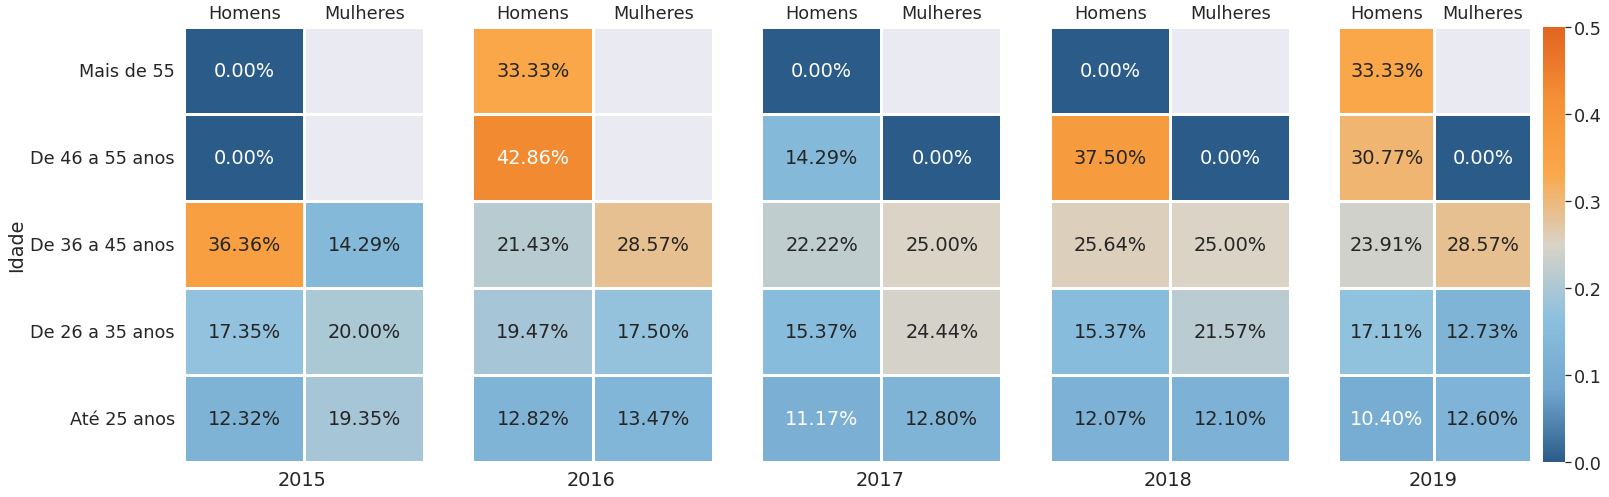
\includegraphics[width=1\textwidth]{figuras/RENOTE/renote.png}
% \caption{Taxa de Evasão Por Gênero e Idade no Ensino Superior.\\Fonte: \cite{santos2022analise}}
% \label{fig:renote}
% \end{figure}


%, desta forma o presente artigo é de contribuição valiosa para a revista Renote(Revista Novas Tecnologias na Educação) pois aborda um problema importante e atual na área de tecnologia e educação e como a Renote tem como foco realizar o compartilhamento de conhecimento cientifico, a abordagem de problemas atuais na área da tecnologia este artigo cumpre o foco da revista.

\section{Trabalho \ref{trab:diversidade}: Panorama da Diversidade}
\label{sec:panorama}

Considerando a importância e o escopo da diversidade apresentada na seção \ref{subsubsec:diversidade}, o trabalho \ref{trab:diversidade} teve como objetivo analisar a diversidade nos cursos da área da computação em universidades públicas de Santa Catarina, e refletir sobre a necessidade de ações para aumentar a diversidade nessas instituições e em outras regiões do Brasil. A coleta de dados abrange o período de 2015 a 2019, onde foi possível identificar que os cursos da área de computação nas universidades públicas de Santa Catarina ainda apresentam uma baixa representatividade de mulheres, pessoas negras e indígenas.


%Portanto, este trabalho tem como foco principal analisar a diversidade nos cursos da área da computação nas universidades públicas de Santa Catarina, com o objetivo de promover uma reflexão sobre a necessidade de ações para aumentar a diversidade nas IESs analisadas e, posteriormente, em outras regiões do Brasil. Para isso, foram coletados dados referentes aos anos de 2015 a 2019, como cor/raça, idade, forma de ingresso, gênero, entre outros. A fundamentação do estudo baseia-se na necessidade de promover a diversidade e a inclusão nos cursos da área da computação, que historicamente têm sido áreas de baixa representatividade de mulheres, pessoas negras e indígenas.

% Em relação ao EduComp, o artigo é relevante para o evento por abordar um tema importante para a área de educação em Computação. Além disso, a discussão sobre a inclusão de grupos historicamente sub-representados nas áreas da computação é pertinente para o evento, que tem como objetivo promover a reflexão sobre os desafios e oportunidades da educação em Computação no Brasil.

\subsection{Resultados}

Através da análise dos dados coletados, foi possível identificar as instituições com maiores e menores porcentagens de diversidade em cada uma das seis categorias avaliadas (gênero, cor e raça, forma de ingresso, reserva de vaga, deficiência e faixa etária). As universidades apresentaram pontos a melhorar em relação à diversidade, sem uma instituição de ensino superior que apareça como mais diversa em todas ou a maioria das características.


%Apesar de a porcentagem de mulheres em cursos de educação superior ser expressiva, sua representatividade ainda é menor nos cursos de tecnologia, onde apenas 17\% dos concluintes são do gênero feminino \cite{santos2022analise}.


%Com a existente necessidade da visualização de dados para uma melhor administração pública e administrativa, é fundamental ter uma ferramenta que permita analisar a evasão, gênero e diversidade, facilitando a identificação de padrões, 
% \label{sec:dataviz}

%%%%%%%%%%%%%%%%%%%%%%%%%%%%%%%%%%%%%%%%%%%%%%%%%%%%%

    % \section{Resultados}
        % \textcolor{red}{verificar se estão querendo mesmo saber!!! ver outros artigos - estão sim, vide: \href{https://sol.sbc.org.br/journals/index.php/reic/article/view/1088/958}{ARTIGO 1} e \href{https://sol.sbc.org.br/journals/index.php/reic/article/view/1747/1596}{ARTIGO 2}}

% A presente seção tratará dos congressos que o grupo publicou alguns dos resultados dos trabalhos citados na seção \ref{sec:trabalhos}. 

% \subsection{Evasão feminina em Ciência da Computação em universidades presenciais de SC}%explicar oq é a renote em ()


% \subsection{Ferramenta de visualização de dados do Censo da Educação Superior do INEP}

\section{Trabalho \ref{trab:dropoutless}: Ferramenta Colaborativa de Predição da Evasão}

A prevenção da evasão é de suma importância, visto que esse fenômeno não afeta apenas o âmbito educacional, mas também repercute em outras áreas da sociedade, como a escassez de mão de obra especializada, o que pode levar a uma redução da competitividade e eficiência das empresas nacionais \cite{mussliner:2021}. Considerando esse cenário, os educadores tem um papel fundamental na prevenção da evasão de estudantes já que dos estudantes diplomados, 80\% afirmaram ter boas relações com os professores, contra apenas 46\% dos evadidos.

Com isso, o Trabalho \ref{trab:dropoutless} tem como objetivo propor uma ferramenta para ajudar professores a prever a evasão de estudantes em suas disciplinas e possibilitar a tomada de ação para a mudança desse cenário. A aplicação busca prever a evasão de forma colaborativa, através da criação coparticipativa de modelos de \textit{Machine Learning} (ML) automatizados, com o auxílio da tecnologia \textit{AutoML}.

% A importância dos educadores na retenção de estudantes é notável, sendo um dos fatores mantenedores dos estudantes no curso visto que 80\% dos estudantes diplomados e apenas 46\% dos estudantes evadidos afirmaram ter boas relações com os professores \cite{silva_rodrigues_brito_frança_2012}. Isso evidencia a necessidade de investir em ações diretas do professor para com seus estudantes.

% O presente artigo tem como objetivo propor uma ferramenta, nomeada Dropoutless, que busca prever a evasão de forma colaborativa, através da criação coparticipativa de modelos de \textit{Machine Learning} (ML) para ajudar professores a prever a evasão de estudantes em suas disciplinas e possibilitar a tomada de ação para a mudança desse cenário. Através da criação de um sistema colaborativo, é possível contornar um dos maiores problemas na utilização de técnicas de ML que é a escassez de dados \cite{bansal:2022}.

% Tendo consciência das possibilidades oferecidas por uma ferramenta de previsão antecipada de evasão, o objetivo deste trabalho é explorar como o uso de um sistema colaborativo pode permitir a criação de modelos de predição de evasão eficazes e de fácil utilização. Através dessa abordagem, busca-se identificar a evasão de estudantes antes que ocorra, possibilitando ações preventivas para evitar que isso aconteça. Assim, foi proposto o desenvolvimento de uma ferrament, utilizou-se de ferramentas de \textit{Machine Learning} automatizadas (AutoML), que são capazes de produzir modelos de predição de forma personalizada, além de tratar das colunas não completamente preenchidas com a entrada automática de números neutros ou zero. Seu uso é possibilitado até mesmo por pessoas que desconhecem a área de computação e inteligência artificial.

\subsection{Resultados}

A plataforma proposta é composta por um sistema de classificação dos modelos de predição, permitindo ao usuário ordená-los de acordo com as métricas de avaliação desejadas. Além disso, é possível filtrar os modelos por meio de \textit{tags}, para exibir apenas aqueles que levam em consideração características específicas na predição. Dessa forma, a ferramenta incentiva a colaboração, possibilitando o uso e aprimoramento contínuo dos modelos desenvolvidos, que se adaptam a diversos cenários acadêmicos e de previsão de evasão.

\section{Conclusão e trabalhos futuros}

A evasão é um grande desafio enfrentado pela educação básica e superior em todo o mundo. Ela é resultado de várias causas que estão relacionadas aos contextos socioeconômicos, políticos e culturais do sistema educacional e das instituições de ensino \cite{silva:2019}. Suas consequências podem ser prejudiciais tanto para o aluno, que pode enfrentar dificuldades para conseguir emprego, quanto para o Estado e o ambiente educacional, representando um desperdício de recursos e esforços.

Dada a importância do tema, as pesquisas realizadas pelo grupo de iniciação científica em evasão ganham notoriedade. Os resultados das análises realizadas nos trabalhos podem auxiliar no desenvolvimento de políticas públicas institucionais ou governamentais, além de também haver a possibilidade de contribuir na tomada de decisões mais assertivas acerca do futuro da educação superior brasileira.

Como perspectivas futuras, o grupo pretende expandir trabalhos anteriores, realizando análises similares em âmbito nacional. Além disso, pretende-se realizar o desenvolvimento de ferramentas que podem auxiliar a democratização do acesso a dados do INEP, para facilitar a realização de outras pesquisas da área de educação com dados públicos. Por fim, o grupo almeja uma pequisa de análise do corpo de docente por um viés de gênero e sua possível relação com a evasão feminina.  

\section{Agradecimentos}

Agradecemos o apoio do Conselho Nacional de Desenvolvimento Científico e Tecnológico (CNPq) 308395/2020-4,  Fundação de Amparo à Pesquisa e Inovação do Estado de Santa Catarina (FAPESC) Nº 027/2020 Apoio a Infraestrutura para Grupos de Pesquisa da UDESC TO n° 2021TR795 e Coordenação de Aperfeiçoamento de Pessoal de Nível Superior - Brasil (CAPES) - Código de Financiamento 001.

% \textcolor{red}{concluímos q nosso grupo eh foda}

%%%%%%%%%%%%%%%%%%%%%%%%%%%%%%%%%%%%%%%%%%%%%%%%%%%%%

\bibliographystyle{sbc}
\bibliography{sbc-template}

\end{document}
